% PLOS ONE manuscript -- PONE-D-26-28965 (revision)
% Based on the official PLOS LaTeX template v3.8 (Apr 2026).
%
% % % % % % % % % % % % % % % % % % % % % % %
%
% THIS IS THE CLEAN MANUSCRIPT.
%
% It contains no revision highlighting: PLOS requires the clean "Manuscript"
% file to be free of tracked changes.
%
% Graphics ARE embedded here, exactly as in initial_submission/main.tex, so the
% working PDF is readable. PLOS requires each figure to be uploaded as an
% individual file (https://journals.plos.org/plosone/s/figures), that project is
% generated by "make prepare-plos-submission", which strips \includegraphics and
% writes figures/Fig<N>.tif. Do not strip the graphics by hand.
%
% The "Revised Manuscript with Track Changes" file is produced from this source
% with latexdiff against the previously submitted version. See ../README.md.
% Do not hand-edit colors into this file.
%
% % % % % % % % % % % % % % % % % % % % % % %
%
% NOTE ON \rev / \revs
% The wrappers \rev{...} and \revs{...} mark passages that were added or
% modified in the first revision round. They are deliberately defined as
% identity macros so that they never render color, while preserving the record
% of which passages changed. Keep them. Do not re-enable the colored versions
% in this file.
%
% % % % % % % % % % % % % % % % % % % % % % %

\documentclass[10pt,letterpaper]{article}
\usepackage[top=0.85in,left=2.75in,footskip=0.75in]{geometry}

% amsmath and amssymb packages, useful for mathematical formulas and symbols
\usepackage{amsmath,amssymb}

% Use adjustwidth environment to exceed column width (see example table in text)
\usepackage{changepage}

% textcomp package and marvosym package for additional characters
\usepackage{textcomp,marvosym}

% cite package, to clean up citations in the main text. Do not remove.
\usepackage{cite}

% Use nameref to cite supporting information files (see Supporting Information section for more info)
\usepackage{nameref,hyperref}

% line numbers
\usepackage[right]{lineno}

% ligatures disabled
\usepackage[nopatch=eqnum]{microtype}
\DisableLigatures[f]{encoding = *, family = * }

% color can be used to apply background shading to table cells only
\usepackage[table]{xcolor}

% array package and table rules
\usepackage{array,booktabs,longtable,float}

% Round-1 revision markers, defined as identity macros so that the clean
% manuscript contains no in-text color (PLOS ONE requirement for the
% unmarked "Manuscript" file). \rev{...} wraps changed paragraphs and
% \revs{...} wraps changed inline fragments such as headings.
\newcommand{\rev}[1]{#1}
\newcommand{\revs}[1]{#1}

% multirow, for scenario cells spanning several rows in the results table
\usepackage{multirow}

% create "+" rule type for thick vertical lines
\newcolumntype{+}{!{\vrule width 2pt}}

% left-aligned fixed-width column, used by the tables in tables/
\newcolumntype{L}[1]{>{\raggedright\arraybackslash}p{#1}}

% create \thickcline for thick horizontal lines of variable length
\newlength\savedwidth
\newcommand\thickcline[1]{%
  \noalign{\global\savedwidth\arrayrulewidth\global\arrayrulewidth 2pt}%
  \cline{#1}%
  \noalign{\vskip\arrayrulewidth}%
  \noalign{\global\arrayrulewidth\savedwidth}%
}

% \thickhline command for thick horizontal lines that span the table
\newcommand\thickhline{\noalign{\global\savedwidth\arrayrulewidth\global\arrayrulewidth 2pt}%
\hline
\noalign{\global\arrayrulewidth\savedwidth}}


% PLOS ONE requires double-spaced manuscript text. The two lines below may be
% commented out while working to keep the PDF compact. The tracked-changes route
% ("make prepare-marked-manuscript") uncomments them again.
\usepackage{setspace}
\doublespacing

% Text layout
\raggedright
\setlength{\parindent}{0.5cm}
\textwidth 5.25in
\textheight 8.75in

% Bold the 'Figure #' in the caption and separate it from the title/caption with a period
% Captions will be left justified
\usepackage[aboveskip=1pt,labelfont=bf,labelsep=period,justification=raggedright,singlelinecheck=off]{caption}
\renewcommand{\figurename}{Fig}

% Please use the included `plos2025.bst` as your BibTeX style
\bibliographystyle{plos2025}

% Remove brackets from numbering in List of References
\makeatletter
\renewcommand{\@biblabel}[1]{\quad#1.}
\makeatother



% Header and Footer with logo
\usepackage{lastpage,fancyhdr,graphicx}
\usepackage{epstopdf}
%\pagestyle{myheadings}
\pagestyle{fancy}
\fancyhf{}
%\setlength{\headheight}{27.023pt}
%\lhead{\includegraphics[width=2.0in]{PLOS-submission.eps}}
\rfoot{\thepage/\pageref{LastPage}}
\renewcommand{\headrulewidth}{0pt}
\renewcommand{\footrule}{\hrule height 2pt \vspace{2mm}}
\fancyheadoffset[L]{2.25in}
\fancyfootoffset[L]{2.25in}
\lfoot{\today}

%% Include all user-defined macros below

%% END MACROS SECTION


\begin{document}
\vspace*{0.2in}

% Title must be 250 characters or less.
\begin{flushleft}
{\Large
\textbf{Evaluation of validation strategies and transferability of EEG attention decoding: a comparative analysis on open datasets} % Please use "sentence case" for title and headings.
}
\newline
% Insert author names, affiliations and corresponding author email (do not include titles, positions, or degrees).
\\
Sanzhar Sovet\textsuperscript{1},
Beibit Abdikenov\textsuperscript{1*},
Manzura Zholdasova\textsuperscript{2,3},
Altyngul Kamzanova\textsuperscript{2},
Medet Mukushev\textsuperscript{1},
Almira Kustubayeva\textsuperscript{2,3}
\\
\bigskip
\textbf{1} Science and Innovation Center ``Artificial Intelligence'', Astana IT University, Astana, Kazakhstan
\\
\textbf{2} Department of Biophysics, Biomedicine, and Neuroscience, Al-Farabi Kazakh National University, Almaty, Kazakhstan
\\
\textbf{3} Brain Institute, Al-Farabi Kazakh National University, Almaty, Kazakhstan
\\
\bigskip

% Use the asterisk to denote corresponding authorship and provide email address in note below.
* beibit.abdikenov@astanait.edu.kz

\end{flushleft}
% Please keep the abstract below 300 words

\section*{Abstract}

\textbf{[TODO --- Write the abstract last. Limit: 300 words.]}

\clearpage
\newgeometry{top=0.85in,left=1in,right=1in,footskip=0.75in}
\linenumbers

% Use "Eq" instead of "Equation" for equation citations.
\section*{Introduction}

Electroencephalography (EEG) is a technique for recording brain activity using multichannel scalp electrodes that measure voltage signals reflecting underlying cognitive processes. It is widely used in neuroscience and brain--computer interface (BCI) research due to its non-invasive nature, high temporal resolution, portability and relatively low cost~\cite{rashid2020bci}. At the same time, EEG signals are inherently noisy, non-stationary, and exhibit high inter-subject and inter-session variability~\cite{wu2022transfer}. In addition, these challenges are compounded by the scarcity of large, diverse, and well-annotated open EEG datasets~\cite{sun2025attention}. Consequently, developing a robust decoding model with strong generalization capabilities across subjects, sessions and tasks remains an open and central challenge~\cite{li2025foundation,wu2022transfer}. One promising approach to solve these problems is transfer learning (TL). TL reuses representations already learned on one or more source problems to reduce the amount of labeled data and training effort a related target problem would otherwise require~\cite{zhang2020transfer}. Its success depends not only on modeling and learning strategies but also on the degree of domain and label compatibility between source and target datasets. 

For cognitive constructs such as attention, this compatibility is especially consequential and difficult to guarantee because attention has always been an ambiguous concept and is not a unitary construct with a single universally accepted operational definition~\cite{sun2025attention,hommel2019noone}. Rather, attention is an umbrella term encompassing a set of partially independent processes and functions, such as selecting relevant information, maintaining focus over time, shifting attention between tasks, and allocating cognitive resources. These processes may operate on both external sensory input and internally represented information, including information maintained in working memory~\cite{hommel2019noone,knudsen2007components,petersen2012attention}. The relative contributions of these processes may vary with task demands, sensory modalities, task goals, experimental instructions, assigned conditions, self-reported assessments, and other aspects of experimental design and label definition. Consequently, experimental paradigms described as measuring ``attention'' may probe non-equivalent configurations of cognitive processes. As a result, different datasets may represent different attention-related cognitive states while assigning them the same nominal labels.

Previous EEG transfer-learning research has been predominantly concerned with cross-subject and cross-session generalization, whereas cross-task, cross-dataset, and cross-paradigm transfer have received comparatively less systematic attention~\cite{wu2022transfer,zhou2022crosstask,song2024signal}. Consequently, systematic empirical evidence for source--target suitability across heterogeneous attention-related EEG datasets and tasks remains limited. Source--target suitability is often motivated conceptually or inferred from nominally aligned labels. This leaves unclear which source--target combinations provide useful zero-shot transfer, how much target discriminability is retained relative to target-specific baselines, and whether transferability is direction-dependent. Establishing such pre-adaptation baselines is necessary to justify source selection and to interpret gains or negative transfer from subsequent transfer-learning and domain-adaptation methods~\cite{zhang2023negative}.

[IN PROGRESS --- This paragraph is retained provisionally. Remove it if suitable experiments comparing operational label mappings cannot be completed.] 

Here, we contribute to addressing this gap by systematically evaluating zero-shot generalization across two technically compatible public EEG datasets spanning multiple tasks and paradigms. We examine both within-dataset baseline performance and transfer across subjects, sessions, trials, tasks, and datasets under a common preprocessing pipeline, compare directed source--target pairs against target-specific baselines, and assess transferability using six decoders ranging from linear and tree-based baselines to deep neural networks. Together, these analyses yield reproducible pre-adaptation benchmarks for evaluating candidate sources and contextualizing both gains and negative transfer produced by subsequent transfer-learning and domain-adaptation methods.


\section*{Open-access datasets}

\subsection*{EEG data for mental attention state detection (Dataset A)}

The dataset described in~\cite{aci2019attention} comprises \textbf{34 EEG recordings} collected from \textbf{five participants} over the course of \textbf{seven days}, with the fifth participant completing only \textbf{six sessions}. During each session, participants operated a virtual train using the \textit{Microsoft Train Simulator}. Each recording lasted approximately \textbf{35 to 55 minutes}. All experiments in this study were performed with healthy volunteer participants chosen among students.

To ensure consistency, all sessions were conducted on the same predefined route, designed to require minimal interaction. This setup constitutes a \textbf{low-intensity control task}, minimizing variability due to task demands and aligning with \textit{naturalistic stimulus-based protocols} as described in~\cite{chen2025hybrid}. Each session was divided into \textbf{three sequential phases}, each designed to reflect a different target mental state: \textbf{\textit{focused}}, \textbf{\textit{unfocused}}, and \textbf{\textit{drowsy}}. The participants simulated these mental states based on standardized instructions provided by the experiment supervisor:

\begin{itemize}
  \item \textbf{Focused (0--10 min):} Participants actively monitored and mentally engaged with the simulator, maintaining sustained attention to the virtual controls and screen events.
  \item \textbf{Unfocused (10--20 min):} Participants disengaged from the task, ceasing interaction and intentionally avoiding attentional focus, while being instructed to keep their eyes open and remain awake.
  \item \textbf{Drowsy (20--30 min):} Participants were allowed to relax, close their eyes, and enter a drowsy or lightly dozing state, simulating reduced cognitive arousal.
\end{itemize}

EEG signals were recorded using a \textbf{modified Emotiv headset}, equipped with wet electrodes and supporting wireless Bluetooth transmission. The device recorded data at a \textbf{sampling rate of 128~Hz} and with a \textbf{voltage resolution of 0.51~$\mu$V}. The dataset includes \textbf{14 EEG channels}, labeled according to the 10--20 international system: AF3, F7, F3, FC5, T7, P7, O1, O2, P8, T8, FC6, F4, F8, and AF4.

\subsection*{SAM-40: dataset of 40-subject EEG recordings (Dataset B)}

The \textbf{SAM-40} dataset, described in~\cite{ghosh2022sam40}, contains EEG recordings from 40 healthy participants (14 females and 26 males) with a mean age of 21.5 years. The purpose of data collection was to investigate short-term stress responses induced by the performance of various cognitive tasks, which correspond to a \textit{continuous cognitive engagement} paradigm as described in~\cite{chen2025hybrid}. The experimental protocol included four conditions:

\begin{itemize}
  \item \textbf{Resting state} --- EEG recording during relaxation while listening to music.
  \item \textbf{Stroop Color-Word Test} --- participants were required to identify the color of the ink in which a word was printed, while ignoring the word's semantic meaning. The task included two types of stimuli: \textit{congruent} (the color name matched the ink color) and \textit{incongruent} (the color name and ink color differed). Each execution of the task included 11 stimuli.
  \item \textbf{Arithmetic problem solving} --- participants mentally solved a mathematical problem and determined whether the presented answer was correct, responding with a ``thumbs up'' or ``thumbs down'' gesture. Each execution of the task included 6 arithmetic stimuli.
  \item \textbf{Mirror Image Recognition} --- participants were shown images and asked to determine whether they were mirror-symmetric or asymmetric, responding with the same gestures. Each execution of the task included 8 images.
\end{itemize}

Each task lasted 25 seconds, with 5-second rest intervals and a 10-second instruction period preceding the next task. After the completion of each trial, participants rated the level of stress experienced for each task on a 10-point scale, where 1 indicated minimal stress and 10 indicated maximal stress. For each participant, three trials were recorded using different sets of stimuli.

EEG signals were recorded using an Emotiv Epoc Flex headset with 32 wet electrodes, labeled according to the international 10--20 system. Data were acquired at a sampling rate of 128~Hz and a voltage resolution of 0.51~$\mu$V. The 32 channels included in the dataset are: Cz, Fz, Fp1, F7, F3, FC1, C3, FC5, FT9, T7, CP5, CP1, P3, P7, PO9, O1, Pz, Oz, O2, PO10, P8, P4, CP2, CP6, T8, FT10, FC6, C4, FC2, F4, F8, and Fp2.

\section*{Methodology}

The methodological design of this study was developed to evaluate the generalizability and transferability of EEG-based attention decoding across different recording conditions, participants, and task paradigms. To this end, we adopted two publicly available datasets that differ in experimental protocols but share compatible technical specifications, which allows for a controlled comparative analysis. \rev{The datasets were harmonized through a binary operational labeling scheme that distinguishes conditions of high protocol-defined task demand from conditions of rest or task disengagement, enabling consistent evaluation across scenarios.} This section outlines the rationale for dataset alignment, the strategies employed for cross-validation, and the experimental settings designed to assess within-dataset performance as well as cross-subject, cross-session, \rev{cross-trial,} cross-task, and cross-dataset generalization.

All experiments were executed through a version-controlled computational workflow. For every run, the workflow stores the resolved configuration of data preparation, validation and model settings together with the run outputs needed to reconstruct the reported evaluation metrics. These records provide run-level provenance for the results and permit the correspondence between a reported metric and the experiment that produced it to be inspected. The complete implementation, experiment configurations and run-level artifacts are available at \url{https://github.com/sovetskiysn/eeg-validation-strategies}.

\subsection*{Dataset alignment and integration rationale}

Effective evaluation of cross-task and cross-dataset generalization relies on the availability of datasets that are compatible both technically and conceptually. In this study, we integrate two publicly available EEG datasets that differ in their original purpose and labeling schemes, yet retain sufficient technical and conceptual compatibility for a meaningful comparison.

A major strength of this dataset combination lies in their acquisition setup. Both datasets were recorded using Emotiv EEG systems with the same sampling rate (128~Hz) and voltage resolution, although their original electrode montages differed (14 versus 32 channels). For cross-dataset analyses, only the 12 channels common to both datasets were retained. Differences in EEG recording systems and electrode configurations can hinder cross-dataset transferability~\cite{lan2019domain}. Restricting the analysis to the shared channels substantially reduces this configuration-related mismatch, although it does not eliminate all acquisition-related distribution shifts. Within the limited set of publicly available datasets suitable for this comparison, this pair offered a comparatively compatible basis for the present comparative evaluation.

The conceptual rationale for combining the datasets rests on the cognitive conditions represented in their respective protocols. The mental attention-state dataset contains explicit attention-state labels (\textit{Focused}, \textit{Unfocused}, and \textit{Drowsy}) collected during a low-interaction simulation task, whereas SAM-40 was originally designed for stress assessment. Both capture cognitive conditions strongly tied to attentional processes. The SAM-40 dataset includes tasks widely recognized in cognitive neuroscience for eliciting high levels of attentional engagement:
\begin{itemize}
    \item \textbf{Stroop Color Test} --- probes both \textit{selective} and \textit{sustained attention}, requiring participants to suppress automatic reading responses and continually focus on the ink color throughout the task~\cite{macleod1991stroop, scarpina2017stroop, esterman2013zone}.
    \item \textbf{Mental arithmetic task} --- demands \textit{sustained internal attention} and working memory for continuous manipulation of numerical information~\cite{grabner2007math, kitaura2017functional}.
    \item \textbf{Mirror image recognition task} --- engages visuospatial processing and requires both \textit{selective} and \textit{sustained attention} to discriminate between symmetric and asymmetric patterns, relying on mental rotation processes that demand continuous cognitive effort~\cite{shepard1971mental, hyun2007visual, tomasino2016mental}.
\end{itemize}

The simulator-based and task-based datasets correspond, respectively, to the \textit{naturalistic stimulus-based protocols} and \textit{continuous cognitive engagement} paradigms described in~\cite{chen2025hybrid}. In the unified labeling scheme, \textit{Rest} and \textit{Unfocused} are treated as low-attention states, whereas \textit{Focused}, \textit{Stroop}, \textit{Arithmetic}, and \textit{Mirror recognition} are treated as high-attention states. The \textit{Drowsy} phase is excluded from this mapping and from all subsequent preprocessing and analyses because permitted eye closure and drowsiness may confound the comparison with differences in arousal, visual input, and ocular activity. This mapping is summarized in Table~\ref{tab:label_mapping}.

\begin{table}[!ht]
\centering
\caption{\textbf{Unified binary attention label mapping across datasets.}}
\label{tab:label_mapping}
\begin{tabular}{|c|c|}
\hline
\textbf{Attention State} & \textbf{Conditions} \\
\hline
High Attention & Focused, Stroop, Arithmetic, Mirror \\
Low Attention  & Unfocused, Rest \\
\hline
\end{tabular}
\end{table}

\subsection*{\revs{Validation strategies}}

\rev{We evaluated the decoders under six validation protocols, each addressing a distinct generalization question. To preserve the independence of the training and test data, all windows originating from the same recording unit were assigned to the same partition. This prevents overlapping windows from being divided between training and test sets, reducing the risk of overly optimistic performance estimates due to temporal autocorrelation between neighboring EEG windows~\cite{chen2025hybrid}. The within-domain baseline estimates performance when training and test data share the same dataset and condition composition but originate from different recording units. The remaining protocols examine whether discriminative performance is retained when training and testing are separated by participant, recording session, repeated trial, task composition, or dataset. These protocols were applied only where the structure of each release supported their interpretation: repeated recording days in the mental attention-state dataset enabled cross-session validation, whereas repeated trials and multiple tasks in SAM-40 enabled cross-trial and cross-task validation. Model fitting was confined to the training data, and the resulting decoder was evaluated on held-out data without target-specific adaptation. Any class imbalance was handled by oversampling the minority class within the training data only, while the test data retained their observed class distribution.}

\textbf{Baseline (within-dataset, within-subject evaluation).}
\rev{Reference performance was estimated using five-fold stratified group cross-validation, separately for the mental attention-state dataset, the complete SAM-40 composition, and each single-task composition of SAM-40. The grouping variable was the physical recording unit: one selected session in the mental attention-state dataset and one trial-level recording unit in SAM-40, comprising all task recordings included in the analysis for that trial. Training and test folds thus shared the dataset and condition composition and could contain data from the same participants, but never from the same recording unit. These estimates serve as within-domain comparators for the transfer protocols. No separate baseline was defined for the two-task composite compositions.}

\textbf{Cross-subject validation.}
\rev{In each leave-one-subject-out fold, the decoder was trained on all selected data from the remaining participants and tested on all selected data from the held-out participant. The resulting performance quantifies zero-shot generalization to an unseen participant.}

\textbf{Cross-session validation.}
\rev{For each participant in the mental attention-state dataset, the decoder was trained on the selected sessions other than one and tested on the held-out session. Participant identity, task protocol, and acquisition system were therefore held constant while the recording day changed. Although individual recordings in SAM-40 are distributed as separate files, the source article describes the three repetitions as trials and does not identify them as distinct recording sessions. SAM-40 was therefore not included in this analysis.}

\textbf{\rev{Cross-trial validation.}}
\rev{To evaluate variability between repetitions of the SAM-40 protocol under a less stringent separation than cross-session validation, one trial at a time was held out within each participant. The decoder was trained on the remaining trials from that participant and tested on the held-out trial, with all selected task recordings and their windows kept together. This protocol measures generalization across repeated acquisitions within the same visit, not across independently recorded sessions.}

\textbf{Cross-task validation.}
\rev{In SAM-40, each task composition represented the same binary contrast of relaxation versus one or two high-demand tasks, rather than classification of task identity. Cross-task transfer therefore asked whether a decoder fitted to this contrast under one task composition retained discriminative performance under another. We evaluated both directions between the three single-task compositions and between single-task and complementary two-task compositions. Single-task targets were interpreted relative to their corresponding within-domain baselines.}

\rev{The cross-task folds were also subject-disjoint. For each fold, the source composition from all but one participant formed the training set, whereas the target composition from the held-out participant formed the test set. The protocol thus evaluates the combined shift to an unseen participant and a different task composition, rather than within-participant transfer between tasks. This distinction prevents participant-specific EEG patterns from contributing to apparent cross-task generalization~\cite{kamrud2021vigilance,ke2021crosstask}.}

\textbf{Cross-dataset validation.}
\rev{To evaluate transfer between datasets, models were trained on all available data from a source composition and tested on a composition from the other dataset, in both transfer directions and without target-specific adaptation. SAM-40 was considered as a complete composition and through its single-task and two-task compositions. Unlike the preceding protocols, cross-dataset validation changes several factors simultaneously, including the participant population, experimental paradigm, recording setup, and condition definitions. It therefore measures transfer under their compound distribution shift rather than attributing a performance change to any single factor~\cite{lan2019domain}. The common sampling rate, harmonized binary labels, and shared 12-channel montage establish a compatible input and prediction space, but do not remove the substantive differences between the two datasets.}

\subsection*{Data preparation}

\rev{A common, deliberately parsimonious preparation pipeline, implemented in
MNE-Python, was applied to both datasets and across all validation protocols.
Its filtering, ICA, channel
alignment and windowing parameters were fixed in advance and were not tuned
separately for a dataset, task composition, validation protocol or decoder. The
purpose was to place recordings in a common input space while limiting
preprocessing itself as an additional source of variation. Differences between
validation results are therefore interpreted against a fixed preparation
procedure.}

\rev{\textbf{Recording and label selection.} Recordings were selected
before signal processing. Following the source study, the first two recording
sessions for each participant in the mental attention-state dataset were
intended for habituation to the simulator and were not included in the
analyses~\cite{aci2019attention}. The \textit{Drowsy} condition was excluded
from the binary classification analysis because participants were
permitted to close their eyes and enter a drowsy state. This condition differs
from the \textit{Focused} and \textit{Unfocused} conditions not only in
protocol-defined task demand, but also in arousal, visual input and ocular
activity. Including it in the low-attention class would therefore confound the
intended contrast, so no drowsy epochs were generated or presented to a
classifier. In contrast, the complete collection of SAM-40 recordings was
retained for analysis. SAM-40 provides the task recordings of each trial as
separate files. Within each scenario, the task recordings selected from one
trial were grouped into a single recording unit, whereas task recordings not
selected by the scenario were not carried forward to later preparation steps.
Accordingly, the binary mapping in Table~\ref{tab:label_mapping} was applied to the
retained recordings from the two datasets.}

\rev{\textbf{Filtering and ICA cleaning.} Processing was performed for
each recording unit, defined by the combination of participant, session and run
identifiers. To prevent preprocessing from becoming an additional source of
variation, we used a deliberately restrained, conventional procedure:
standard filtering followed by ICA-based artifact cleaning. Keeping
preparation deliberately simple allows differences in performance to be
interpreted primarily in relation to the recordings and validation protocols,
rather than to a complex preparation pipeline. Within each recording unit, EEG channels were
notch-filtered at 50~Hz,
band-pass filtered from 0.5 to 45~Hz and rereferenced to the average reference.
Artifact removal used FastICA fitted to the concatenated recordings of each
recording unit, retaining components that explained 99\% of the variance. The
decomposition was fitted to a 1--45~Hz copy of the prepared signal and then
applied to each recording separately, while the analysis signal retained the
0.5--45~Hz band-pass. Ocular components were identified with F3, F4, F7 and F8
as EOG-proxy channels at a z-score threshold of 2.4 and removed. The ICA random
state was fixed by the experiment configuration. When an excluded condition
occurred as a block within an otherwise selected continuous recording, it
remained available for ICA fitting but was omitted from window generation and
the analysis sets. In the mental attention-state dataset, this applied to the
\textit{Drowsy} block.}

\rev{\textbf{Channel alignment and window segmentation.} After signal cleaning, each
recording was restricted to the 12 channels shared by
the two datasets: F3, F4, F7, F8, FC5, FC6, O1, O2, P7, P8, T7 and T8. Each
retained labelled block was segmented into 5-s windows with 0.5-s overlap.
Every retained window inherited the label of its source block and metadata identifying its
dataset, participant, session, task, run, recording unit and temporal onset.
The recording-unit identifier was used by the validation protocols to ensure
that all overlapping windows from a unit remained on the same side of a split.}

\subsection*{\revs{Models}}

\rev{We evaluated five classifiers rather than relying on a single decoder to
test whether the conclusions are robust to a change in modelling assumptions.
This makes the decoder an explicit factor of the design: a difference between
validation protocols that is reproduced across models is more credibly
attributed to the data and evaluation protocol than to the idiosyncrasies of
one learner. The selected models span three major families used in EEG
decoding: linear and tree-based traditional machine-learning models, and
deep-learning architectures. We place particular emphasis on deep learning
because these models learn task-relevant representations directly from the
channel-by-time EEG windows, reducing reliance on a manually specified feature
set. Hyperparameters were fixed \textit{a priori} for each model and held
constant across validation protocols and experimental runs; they were not tuned
to an individual protocol or run and are recorded in full in the configuration
stored with every run. All models were trained to predict whether a window
belonged to a high-demand or a low-demand condition in the sense of
Table~\ref{tab:label_mapping}, and not to predict a level of attention.}

\textbf{Traditional machine learning.}
\rev{Logistic regression provides a
transparent linear baseline and represents the simplest decision rule supported
by the fixed feature representation. XGBoost~\cite{chen2016xgboost} represents
tree-based ensemble learning, allowing nonlinear relations and feature
interactions to be modelled within the same representation. It was also the
decoder used in the originally submitted version of this study, preserving a
direct point of comparison with those results. Both models received a fixed,
label-free feature representation comprising log band power in delta
(0.5--4~Hz), theta (4--8~Hz), alpha (8--13~Hz), beta (13--30~Hz) and gamma
(30--45~Hz), together with spectral, approximate, sample and
singular-value-decomposition entropy, mean, standard deviation, variance,
skewness and kurtosis, computed for each channel. Feature extraction contained
no trainable transformation. Transformations that learn from data were fitted
within each training fold only: logistic-regression features were standardized
on the training data, whereas XGBoost received unscaled features.}

\textbf{Deep learning.}
\rev{The remaining three classifiers operate directly on the prepared
channel-by-time EEG windows and learn their representations during training.
\textit{ShallowFBCSPNet}~\cite{schirrmeister2017deep} is a shallow
convolutional neural network designed to emulate the main operations of the
filter-bank common spatial pattern (FBCSP) pipeline within a trainable model.
It first applies temporal convolution and spatial filtering across channels,
then uses a squaring nonlinearity, mean pooling and a logarithmic activation to
form band-power-like features. Thus, its inductive bias reflects a conventional
EEG decoding approach, while its filters are optimized jointly with the
classifier.

\textit{EEGNet}~\cite{lawhern2018eegnet} is a compact convolutional neural
network designed specifically for EEG. Its temporal convolutions learn filters
over time, depthwise convolutions learn spatial filters across electrodes for
each temporal feature map, and separable convolutions combine these learned
features efficiently. This factorized design substantially limits the number
of trainable parameters while retaining separate temporal and spatial feature
learning, making EEGNet the smallest network in the present comparison.

\textit{EEG Conformer}~\cite{song2023conformer} combines a convolutional
front end with a Transformer encoder. The convolutional module forms local
temporal and spatial features and converts them into a sequence of embeddings;
self-attention in the Transformer then models global dependencies between these
embeddings. It therefore complements the local receptive fields of convolution
with a mechanism for relating EEG patterns over longer time spans. The only
fixed input transformation for the deep-learning models was conversion from
volts to microvolts. The networks were trained from scratch. No pretrained
weights were used.}

\textbf{[TODO --- Which decoder carries the Results narrative?]}

\section*{Results}

\textbf{[TODO --- This section is preliminary and requires substantial further development before submission.]}

Table~\ref{tab:results_logistic} first gives the complete numerical results
for spectral logistic regression across all validation scenarios, including
balanced accuracy, macro F1, MCC, ROC--AUC and per-class recall. Figures~\ref{fig:all_scenarios_logistic},
\ref{fig:all_scenarios_xgboost} and \ref{fig:cross_subject_model_comparison}
give the corresponding main-text graphical summaries: the per-protocol results
for spectral logistic regression and XGBoost, followed by the cross-subject
comparison across all decoders and both datasets. The three neural-network
per-protocol plots are reported in \nameref{S1_Fig}, \nameref{S2_Fig} and
\nameref{S3_Fig}, respectively. The complete per-scenario numerical outputs
for all five decoders are provided in
\nameref{S1_Table_Logistic},
\nameref{S2_Table_XGBoost}, \nameref{S3_Table_EEGNet},
\nameref{S4_Table_ShallowNet} and \nameref{S5_Table_EEGConformer}.

% This source template is filled by python_project/src/analysis.py.
% Generated tables belong in latex_documents/revision/manuscript_clean/tables/.
\begingroup
\singlespacing
\normalsize
% Add visible, compact spacing around task-transition arrows.
\def\!{\mskip4mu}
% Distribute the remaining width across the 12 internal cell-side paddings.
\setlength{\tabcolsep}{\textwidth}
\addtolength{\tabcolsep}{-12.5cm}
\setlength{\tabcolsep}{0.0833333\tabcolsep}
\renewcommand{\arraystretch}{1.0}
\begin{table}[H]
\centering
\caption{\textbf{Performance metrics across experimental scenarios.}}
\label{tab:results_logistic}
\begin{tabular}{@{}>{\fontsize{8}{9}\selectfont\raggedright\arraybackslash}m{1.9cm}@{\hspace{\tabcolsep}}>{\fontsize{8}{9}\selectfont\raggedright\arraybackslash}m{4.2cm}>{\fontsize{8}{9}\selectfont\centering\arraybackslash}m{1.4cm}>{\fontsize{8}{9}\selectfont\centering\arraybackslash}m{0.9cm}>{\fontsize{8}{9}\selectfont\centering\arraybackslash}m{0.7cm}>{\fontsize{8}{9}\selectfont\centering\arraybackslash}m{1.1cm}>{\fontsize{8}{9}\selectfont\centering\arraybackslash}m{2.3cm}@{}}
\hline
{\fontsize{9}{10}\selectfont Scenario} & {\fontsize{9}{10}\selectfont Validation method} & {\fontsize{9}{10}\selectfont Balanced Accuracy} & {\fontsize{9}{10}\selectfont Macro F1} & {\fontsize{9}{10}\selectfont MCC} & {\fontsize{9}{10}\selectfont ROC AUC} & {\fontsize{9}{10}\selectfont Per-class Recall (Low/High)} \\
\hline
\multirow{5}{=}{Baseline (within)} & Stratified K-fold(Full A) & 0.62 & 0.62 & 0.23 & 0.67 & 0.62/0.61 \\
 & Stratified K-fold(Full B) & 0.61 & 0.58 & 0.20 & 0.65 & 0.60/0.63 \\
 & Stratified K-fold(B: Stroop) & 0.64 & 0.63 & 0.28 & 0.69 & 0.53/0.74 \\
 & Stratified K-fold(B: Arithmetic) & 0.59 & 0.59 & 0.18 & 0.62 & 0.54/0.63 \\
 & Stratified K-fold(B: Mirror) & 0.60 & 0.59 & 0.20 & 0.66 & 0.48/0.71 \\
\hline
\multirow{2}{=}{Cross-subject} & Leave-one-subject-out(Full A) & 0.53 & 0.53 & 0.06 & 0.56 & 0.47/0.59 \\
 & Leave-one-subject-out(Full B) & 0.57 & 0.56 & 0.13 & 0.61 & 0.45/0.69 \\
\hline
Cross-session & Leave-one-session-out(Full A) & 0.59 & 0.59 & 0.19 & 0.62 & 0.54/0.65 \\
\hline
\multirow{12}{=}{Cross-task (Dataset~B)} & Stroop$\!\rightarrow\!$Arithmetic & 0.54 & 0.54 & 0.08 & 0.55 & 0.49/0.59 \\
 & Stroop$\!\rightarrow\!$Mirror & 0.56 & 0.56 & 0.12 & 0.58 & 0.49/0.63 \\
 & Arithmetic$\!\rightarrow\!$Stroop & 0.58 & 0.56 & 0.18 & 0.64 & 0.35/0.81 \\
 & Arithmetic$\!\rightarrow\!$Mirror & 0.57 & 0.55 & 0.14 & 0.60 & 0.40/0.74 \\
 & Mirror$\!\rightarrow\!$Stroop & 0.59 & 0.57 & 0.20 & 0.63 & 0.38/0.81 \\
 & Mirror$\!\rightarrow\!$Arithmetic & 0.55 & 0.54 & 0.09 & 0.56 & 0.42/0.67 \\
\cmidrule{2-7}
 & Arithmetic+Mirror$\!\rightarrow\!$Stroop & 0.59 & 0.58 & 0.19 & 0.64 & 0.43/0.75 \\
 & Stroop+Mirror$\!\rightarrow\!$Arithmetic & 0.54 & 0.54 & 0.07 & 0.56 & 0.51/0.56 \\
 & Stroop+Arithmetic$\!\rightarrow\!$Mirror & 0.57 & 0.57 & 0.14 & 0.59 & 0.51/0.62 \\
 & Stroop$\!\rightarrow\!$Arithmetic+Mirror & 0.55 & 0.55 & 0.11 & 0.58 & 0.45/0.66 \\
 & Arithmetic$\!\rightarrow\!$Stroop+Mirror & 0.56 & 0.56 & 0.14 & 0.62 & 0.33/0.80 \\
 & Mirror$\!\rightarrow\!$Stroop+Arithmetic & 0.58 & 0.58 & 0.16 & 0.61 & 0.37/0.78 \\
\hline
\multirow{14}{=}{Cross-dataset} & Full A$\!\rightarrow\!$Full B & 0.52 & 0.33 & 0.05 & 0.56 & 0.89/0.16 \\
 & Full B$\!\rightarrow\!$Full A & 0.47 & 0.45 & -0.06 & 0.48 & 0.66/0.29 \\
\cmidrule{2-7}
 & Full A$\!\rightarrow\!$Stroop & 0.46 & 0.37 & -0.13 & 0.47 & 0.81/0.10 \\
 & Stroop$\!\rightarrow\!$Full A & 0.47 & 0.47 & -0.05 & 0.48 & 0.58/0.37 \\
 & Full A$\!\rightarrow\!$Arithmetic & 0.51 & 0.45 & 0.04 & 0.53 & 0.85/0.18 \\
 & Arithmetic$\!\rightarrow\!$Full A & 0.47 & 0.45 & -0.07 & 0.48 & 0.65/0.29 \\
 & Full A$\!\rightarrow\!$Mirror & 0.47 & 0.41 & -0.07 & 0.50 & 0.80/0.14 \\
 & Mirror$\!\rightarrow\!$Full A & 0.46 & 0.45 & -0.08 & 0.47 & 0.61/0.32 \\
\cmidrule{2-7}
 & Full A$\!\rightarrow\!$Stroop+Arithmetic & 0.47 & 0.32 & -0.09 & 0.48 & 0.82/0.11 \\
 & Stroop+Arithmetic$\!\rightarrow\!$Full A & 0.47 & 0.45 & -0.07 & 0.48 & 0.65/0.28 \\
 & Full A$\!\rightarrow\!$Stroop+Mirror & 0.47 & 0.32 & -0.08 & 0.49 & 0.84/0.11 \\
 & Stroop+Mirror$\!\rightarrow\!$Full A & 0.47 & 0.45 & -0.06 & 0.48 & 0.65/0.29 \\
 & Full A$\!\rightarrow\!$Arithmetic+Mirror & 0.52 & 0.38 & 0.04 & 0.55 & 0.87/0.16 \\
 & Arithmetic+Mirror$\!\rightarrow\!$Full A & 0.47 & 0.44 & -0.07 & 0.48 & 0.68/0.26 \\
\hline
\end{tabular}
\normalsize
\begin{flushleft}
\textit{Note.} Per-class recall is reported as Low/High. MCC, Matthews correlation coefficient; ROC-AUC, area under the receiver operating characteristic curve. Dashes indicate values to be filled.
\end{flushleft}
\end{table}
\endgroup


For spectral logistic regression, within-dataset balanced accuracy was
0.59--0.64, while the cross-subject estimates were 0.53 for Dataset~A and
0.57 for Dataset~B. Cross-session and cross-trial estimates were 0.59 and
0.61, respectively. Cross-task transfer ranged from 0.54 to 0.59, whereas
cross-dataset transfer was at or below chance in several directed
source--target pairs (0.46--0.52, Fig.~\ref{fig:all_scenarios_logistic}).

\begin{figure}[H]
\centering
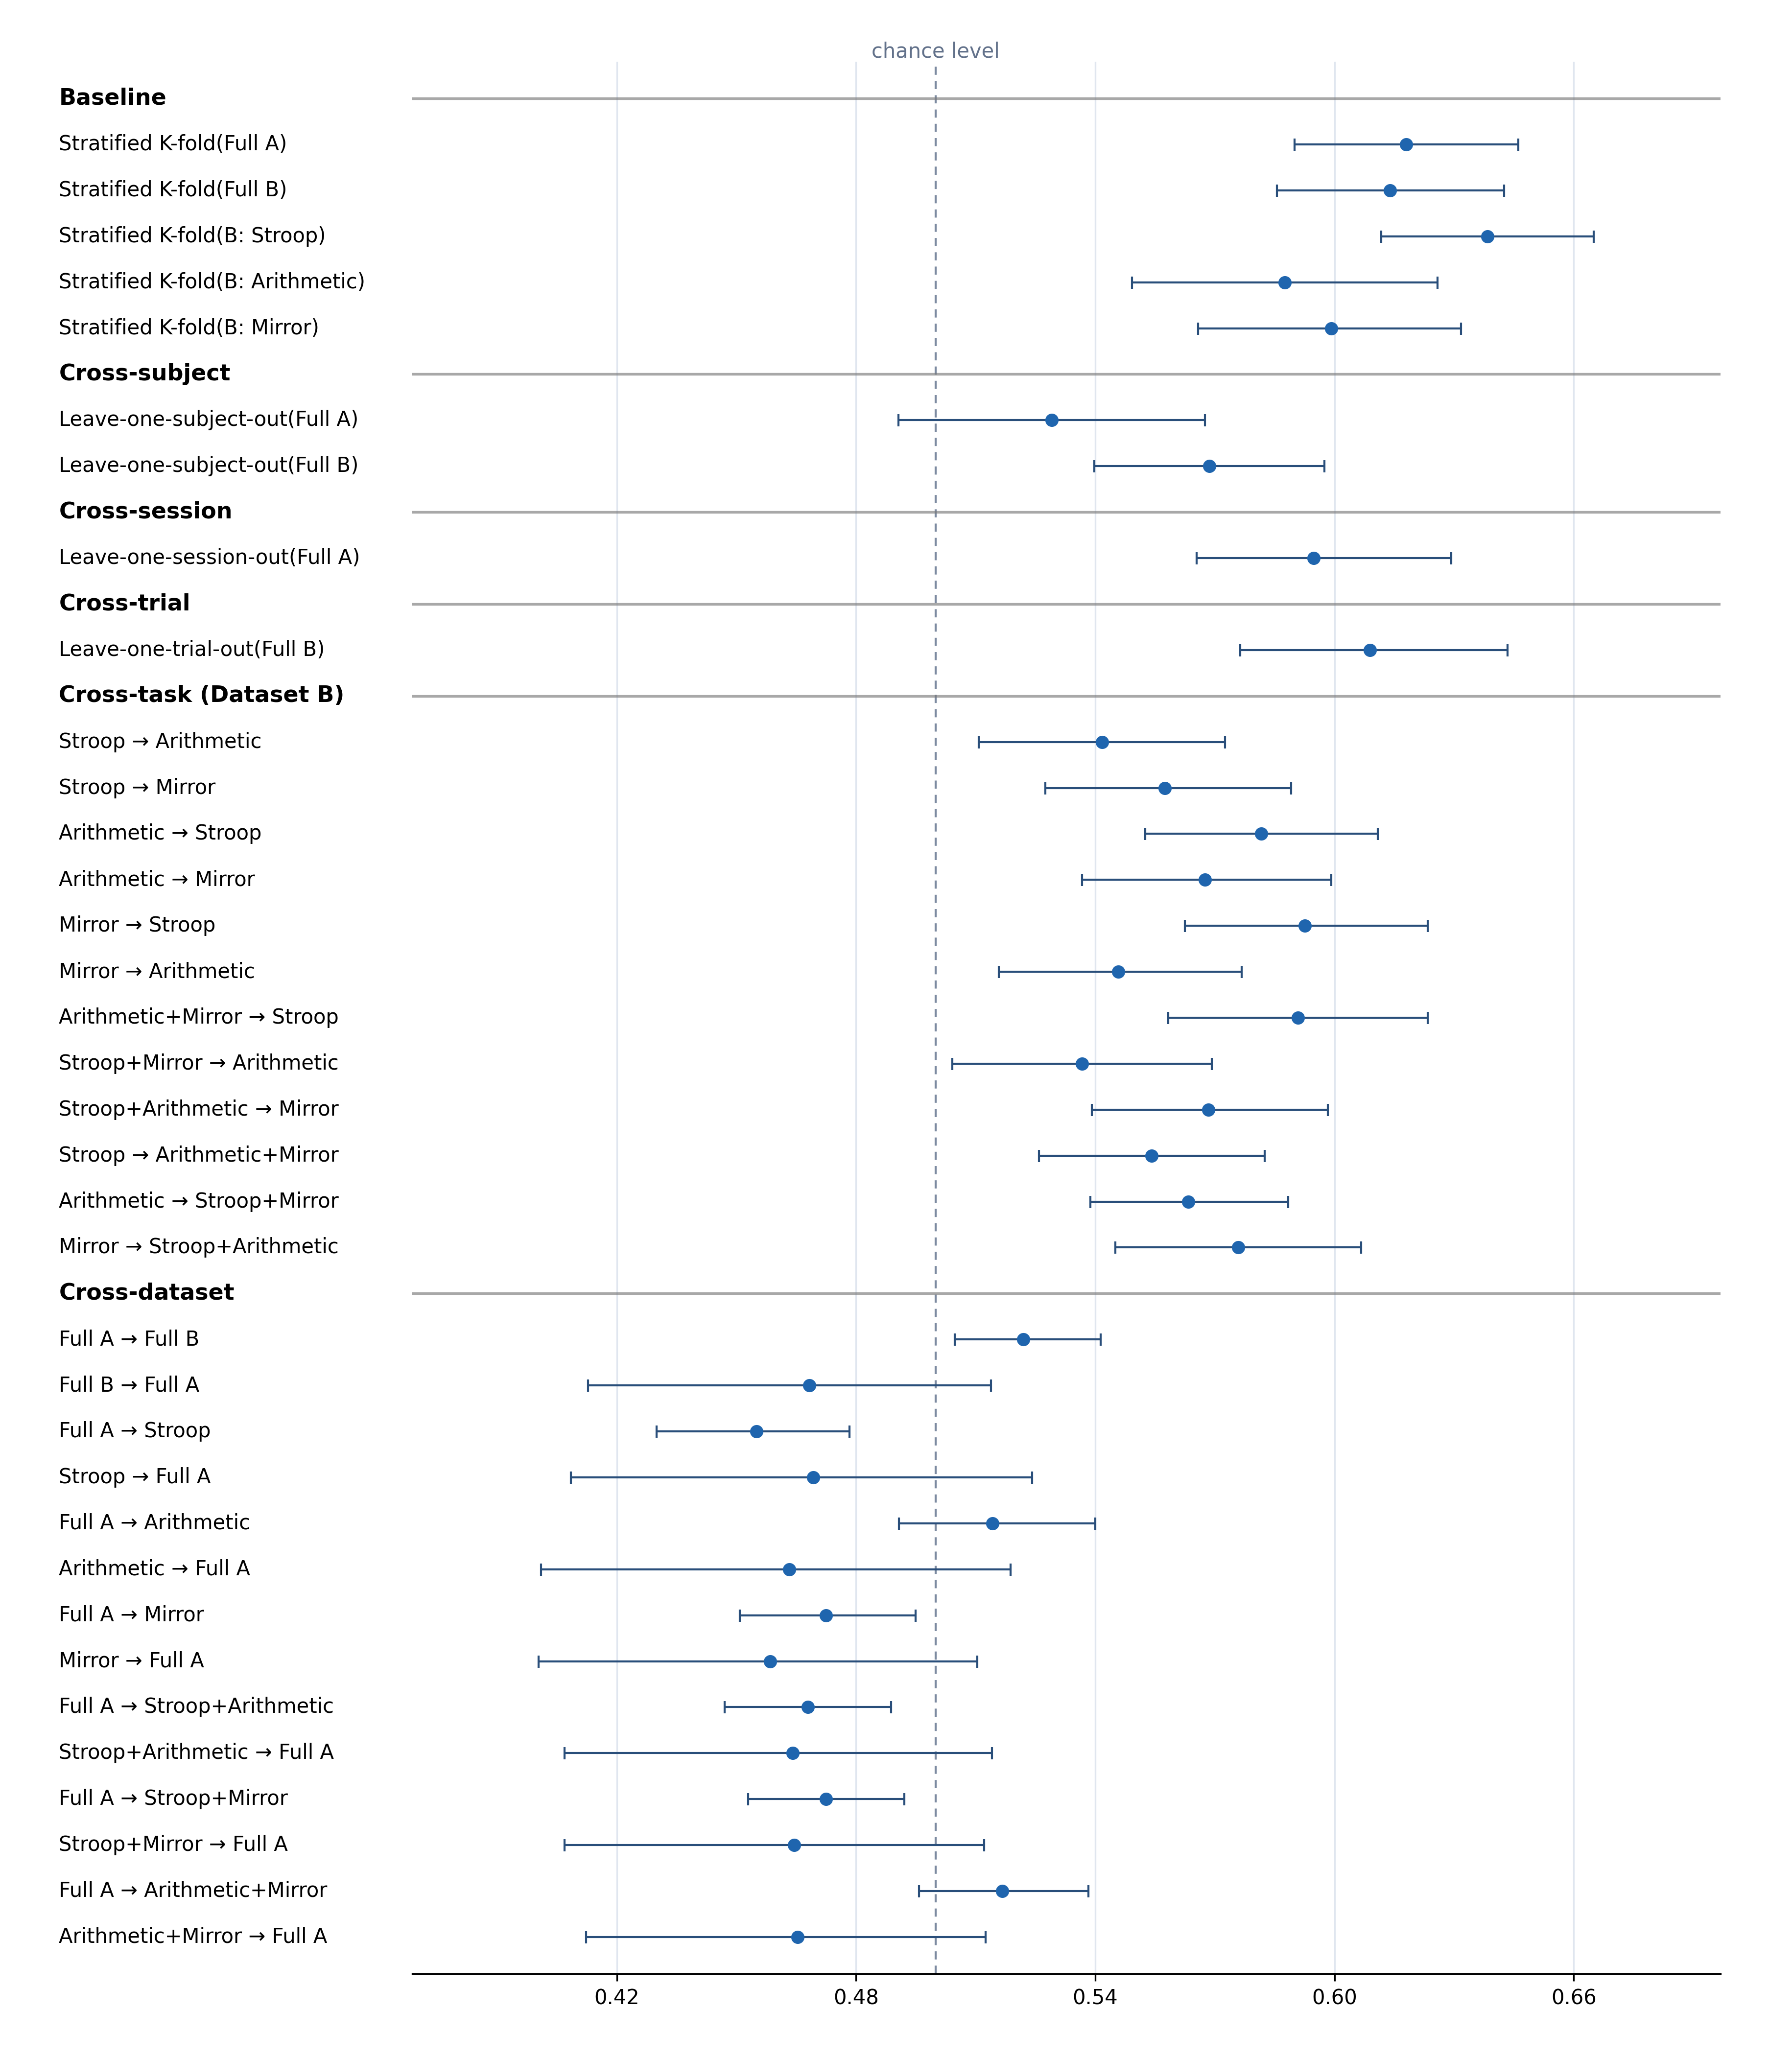
\includegraphics[width=\textwidth,height=0.88\textheight,keepaspectratio]{figures/main/fig1_logistic_regression_all_scenarios.png}
\caption{\textbf{Balanced accuracy across validation protocols for spectral logistic regression.} Points show the estimates plotted by the analysis workflow and horizontal bars show their plotted uncertainty intervals. The dashed vertical line marks chance-level balanced accuracy (0.50). Results are grouped by baseline, cross-subject, cross-session, cross-trial, cross-task and cross-dataset protocols.}
\label{fig:all_scenarios_logistic}
\end{figure}

\begin{figure}[H]
\centering
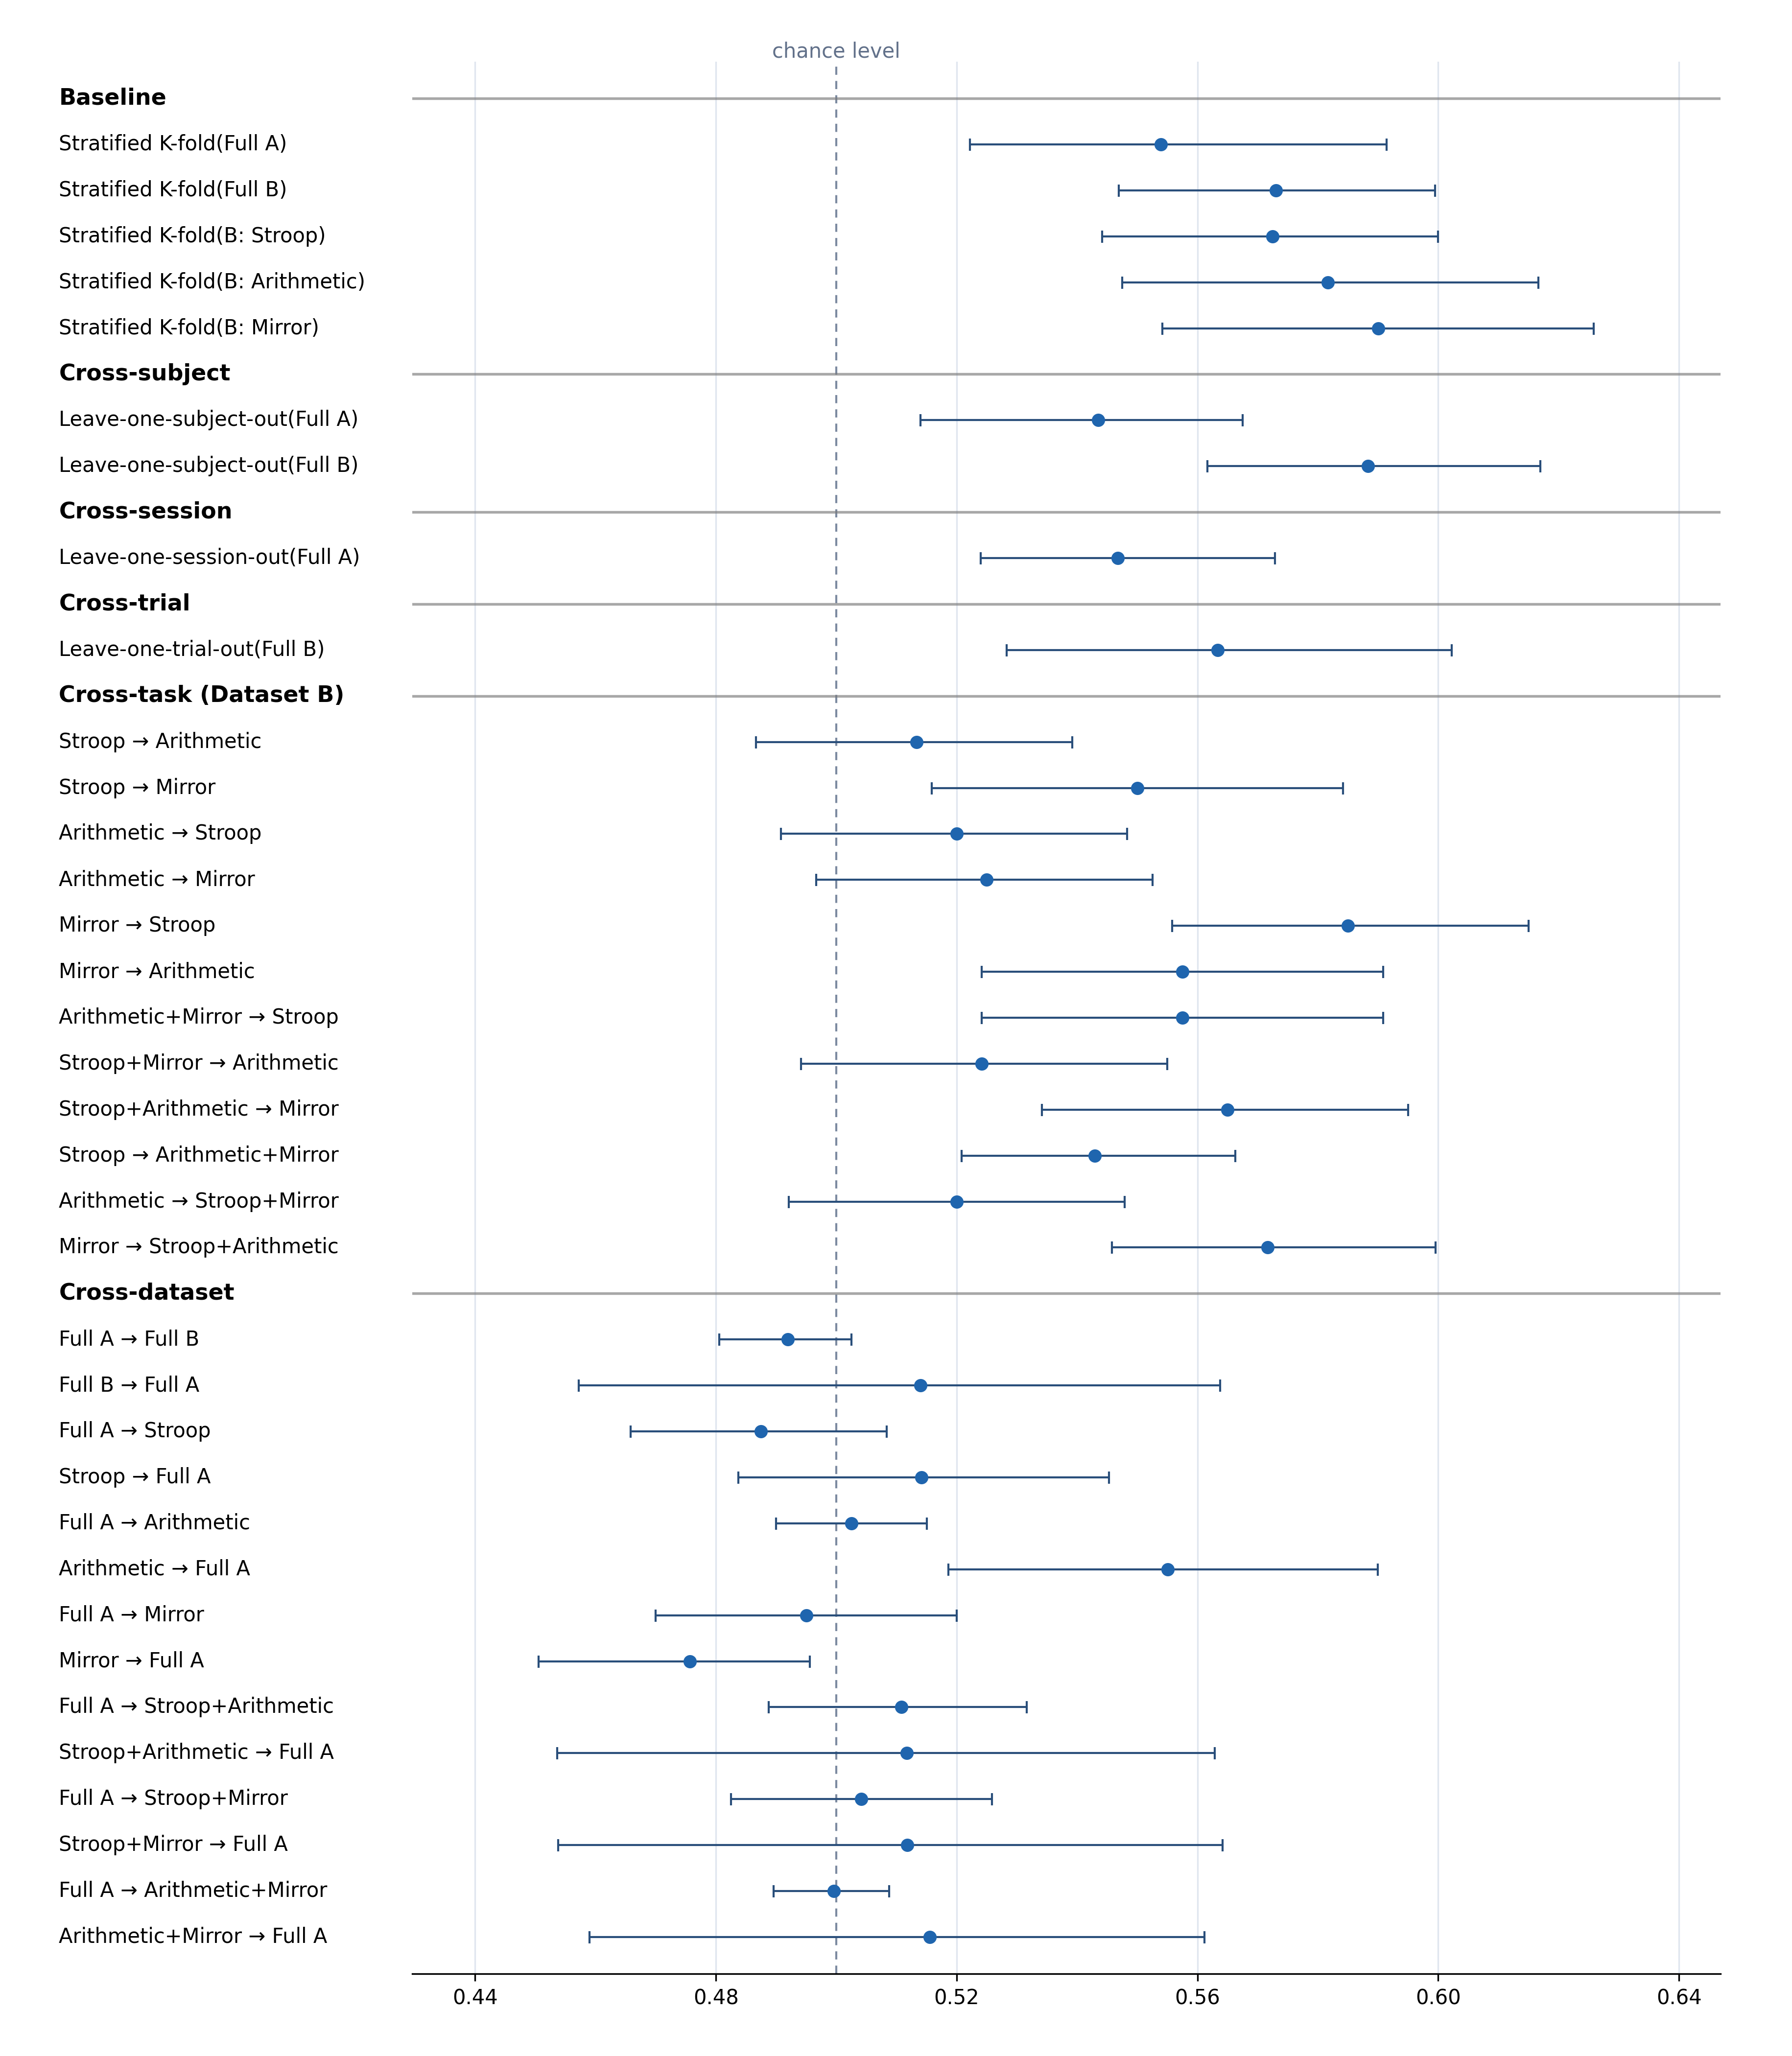
\includegraphics[width=\textwidth,height=0.88\textheight,keepaspectratio]{figures/main/xgboost_all_scenarios.png}
\caption{\textbf{Balanced accuracy across validation protocols for XGBoost.} Points show the estimates plotted by the analysis workflow and horizontal bars show their plotted uncertainty intervals. The dashed vertical line marks chance-level balanced accuracy (0.50). Results are grouped by baseline, cross-subject, cross-session, cross-trial, cross-task and cross-dataset protocols.}
\label{fig:all_scenarios_xgboost}
\end{figure}

\begin{figure}[H]
\centering

\includegraphics[width=\textwidth,height=0.72\textheight,keepaspectratio]{figures/main/cross_subject_model_comparison.png}
\caption{\textbf{Cross-subject balanced accuracy by decoder and dataset.} Each point summarizes the cross-subject balanced-accuracy estimate for one decoder--dataset combination. The dashed line marks chance (0.50).}
\label{fig:cross_subject_model_comparison}
\end{figure}

\section*{Discussion}

\textbf{[TODO --- This section is preliminary and requires substantial further development before submission.]}

This study provides a zero-shot, pre-adaptation benchmark for the extent to
which a decoder trained on one set of EEG recordings can retain
discriminability when the source of variation changes. The comparison treats
the validation protocol and the decoder as design factors: the same fixed
preparation procedure and six decoders, from spectral logistic regression and
XGBoost to four neural architectures, were evaluated across the protocols that
each dataset supports. The resulting estimates are therefore not a competition
for the largest within-dataset score. Instead, they provide a reference against
which a later adaptation or personalization method can be assessed, including
the possibility of negative transfer.

For spectral logistic regression, the within-dataset references were modestly
above chance (balanced accuracy 0.59--0.64), and performance was lower under
the cross-subject protocol for both datasets (0.53 and 0.57). The
cross-session estimate for Dataset~A (0.59) and the cross-trial estimate for
Dataset~B (0.61) show that these sources of variation should not be conflated
with transfer to a new participant or a new task. Subject-disjoint cross-task
estimates in Dataset~B ranged from 0.54 to 0.59. They quantify the retention
of the specified binary contrast when both the participant and task
composition change. They do not isolate a task effect or establish that two
tasks recruit the same cognitive mechanism. The cross-dataset estimates were
at or below chance for several directed source--target pairs (0.46--0.52),
which makes directionality and source--target compatibility central practical
considerations for zero-shot use.

The interpretation of these findings is necessarily limited by the labels.
In both datasets, the class is assigned by the experimental protocol: it
contrasts a condition with higher protocol-defined task demand against rest or
an unfocused condition. It is not an independent measurement of an
individual's level of attention. Accordingly, the results show limited
transferability of this operational contrast between the available datasets
and paradigms. They neither demonstrate the absence of invariant neural
markers of attention nor establish an upper bound on what a different decoder
could achieve. Excluding the drowsy condition avoids one important difference
in arousal, eye closure and ocular activity, but it does not eliminate other
differences in sensory input, task demands, stress, working-memory demands or
time-on-task between the retained conditions.

Several further limitations delimit the benchmark. Only two heterogeneous
open datasets were available for the cross-dataset comparison, and harmonizing
them required restriction to 12 shared channels. This improves input
compatibility while reducing spatial information and limiting the stability of
ICA-based artifact removal. The fixed preparation pipeline and model settings
were chosen to make protocol comparisons consistent, not to optimize each
source--target pair. In particular, this study does not test domain adaptation,
target-specific calibration or personalization, so its cross-dataset estimates
are pre-adaptation references rather than the expected performance of an
adapted system. Finally, the present evaluation does not identify which signal
features drive individual decisions. It therefore cannot attribute transfer
failure to a particular neural, ocular, muscular or other physiological source.
Future work should combine leakage-resistant, subject-disjoint evaluation with
adaptation and diagnostic analyses, and should use datasets in which the target
state is measured independently of the condition used to elicit it.

\section*{Conclusion}

\textbf{[TODO --- This section is preliminary and requires substantial further development before submission.]}

This work benchmarks zero-shot EEG decoding across within-dataset,
cross-subject, cross-session, cross-trial, cross-task and cross-dataset
protocols using six fixed decoders. Its main result is not that a particular
model decodes attention, but that the discriminability of the available
protocol-defined high-demand versus low-demand contrast depends strongly on
how the training and test recordings were obtained. In particular, several
cross-dataset transfers were at or below chance despite channel alignment and
common preprocessing. These estimates establish a pre-adaptation reference for
future transfer-learning and personalization methods. Progress toward
cross-paradigm decoding will also require datasets that establish the target
state independently of the task used to induce it, for example through
concurrent behavioural, validated self-report or external physiological
measurements.

% PLOS ONE ending sections, in the required order:
%   Acknowledgments -> References -> Supporting information captions
% (https://journals.plos.org/plosone/s/submission-guidelines)
%
% The "Funding" section that appeared in the submitted version has been removed.
% PLOS states: "Do not include funding sources in the Acknowledgments or anywhere
% else in the manuscript file. Funding information should only be entered in the
% financial disclosure section" of Editorial Manager. The funder, grant number
% BR27198099 and the Role of Funder statement are carried in
% submission_metadata.md instead.

\textbf{[TODO --- Add acknowledgments if applicable.]}

\nolinenumbers

\bibliography{refs}

\section*{Supporting information}

\paragraph*{S1 Fig.}
\label{S1_Fig}
{\bf EEGNet balanced accuracy across validation protocols.} The per-protocol
EEGNet plot uses the same point, interval and chance-line conventions as
Fig.~\ref{fig:all_scenarios_logistic}.

\paragraph*{S2 Fig.}
\label{S2_Fig}
{\bf ShallowFBCSPNet balanced accuracy across validation protocols.} The
per-protocol ShallowFBCSPNet plot uses the same point, interval and chance-line
conventions as Fig.~\ref{fig:all_scenarios_logistic}.

\paragraph*{S3 Fig.}
\label{S3_Fig}
{\bf EEGConformer balanced accuracy across validation protocols.} The
per-protocol EEGConformer plot uses the same point, interval and chance-line
conventions as Fig.~\ref{fig:all_scenarios_logistic}.

\clearpage
\subsection*{Supporting-information figure previews}

\noindent\textbf{S1 Fig. EEGNet balanced accuracy across validation protocols.}
\begin{center}
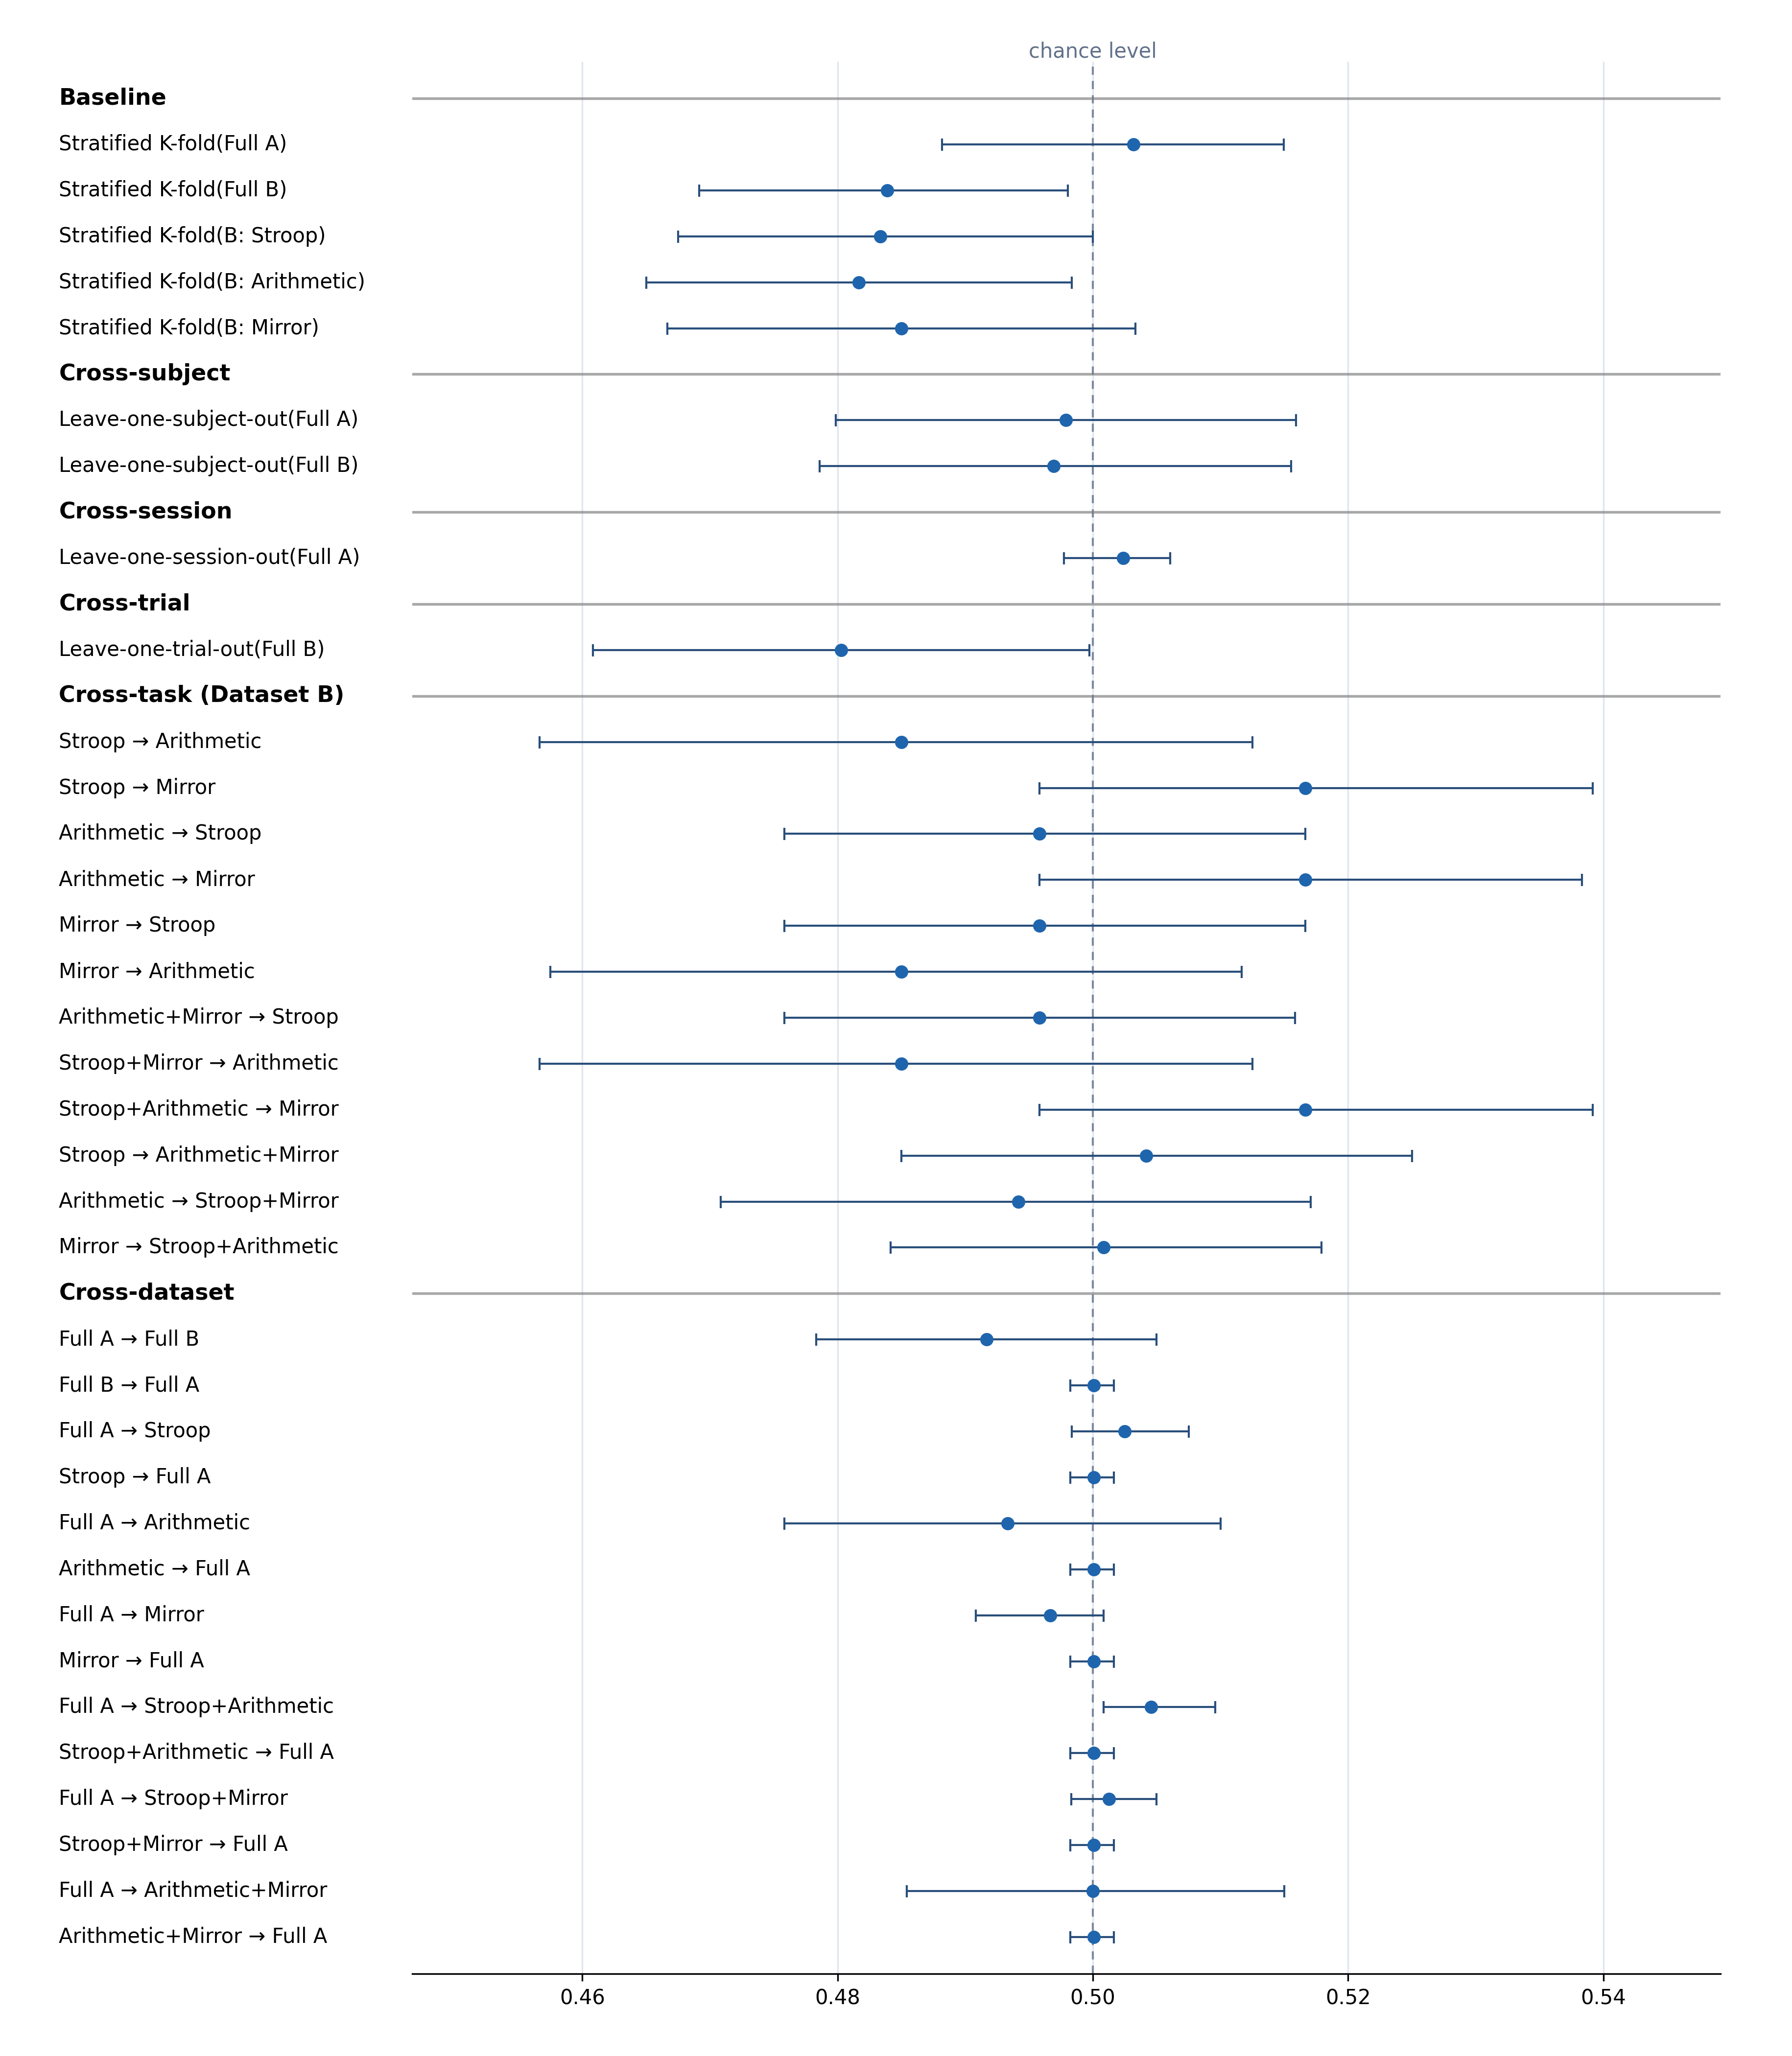
\includegraphics[width=\textwidth,height=0.88\textheight,keepaspectratio]{figures/supplementary/S3_fig_eegnet_all_scenarios.png}
\end{center}

\clearpage
\noindent\textbf{S2 Fig. ShallowFBCSPNet balanced accuracy across validation protocols.}
\begin{center}
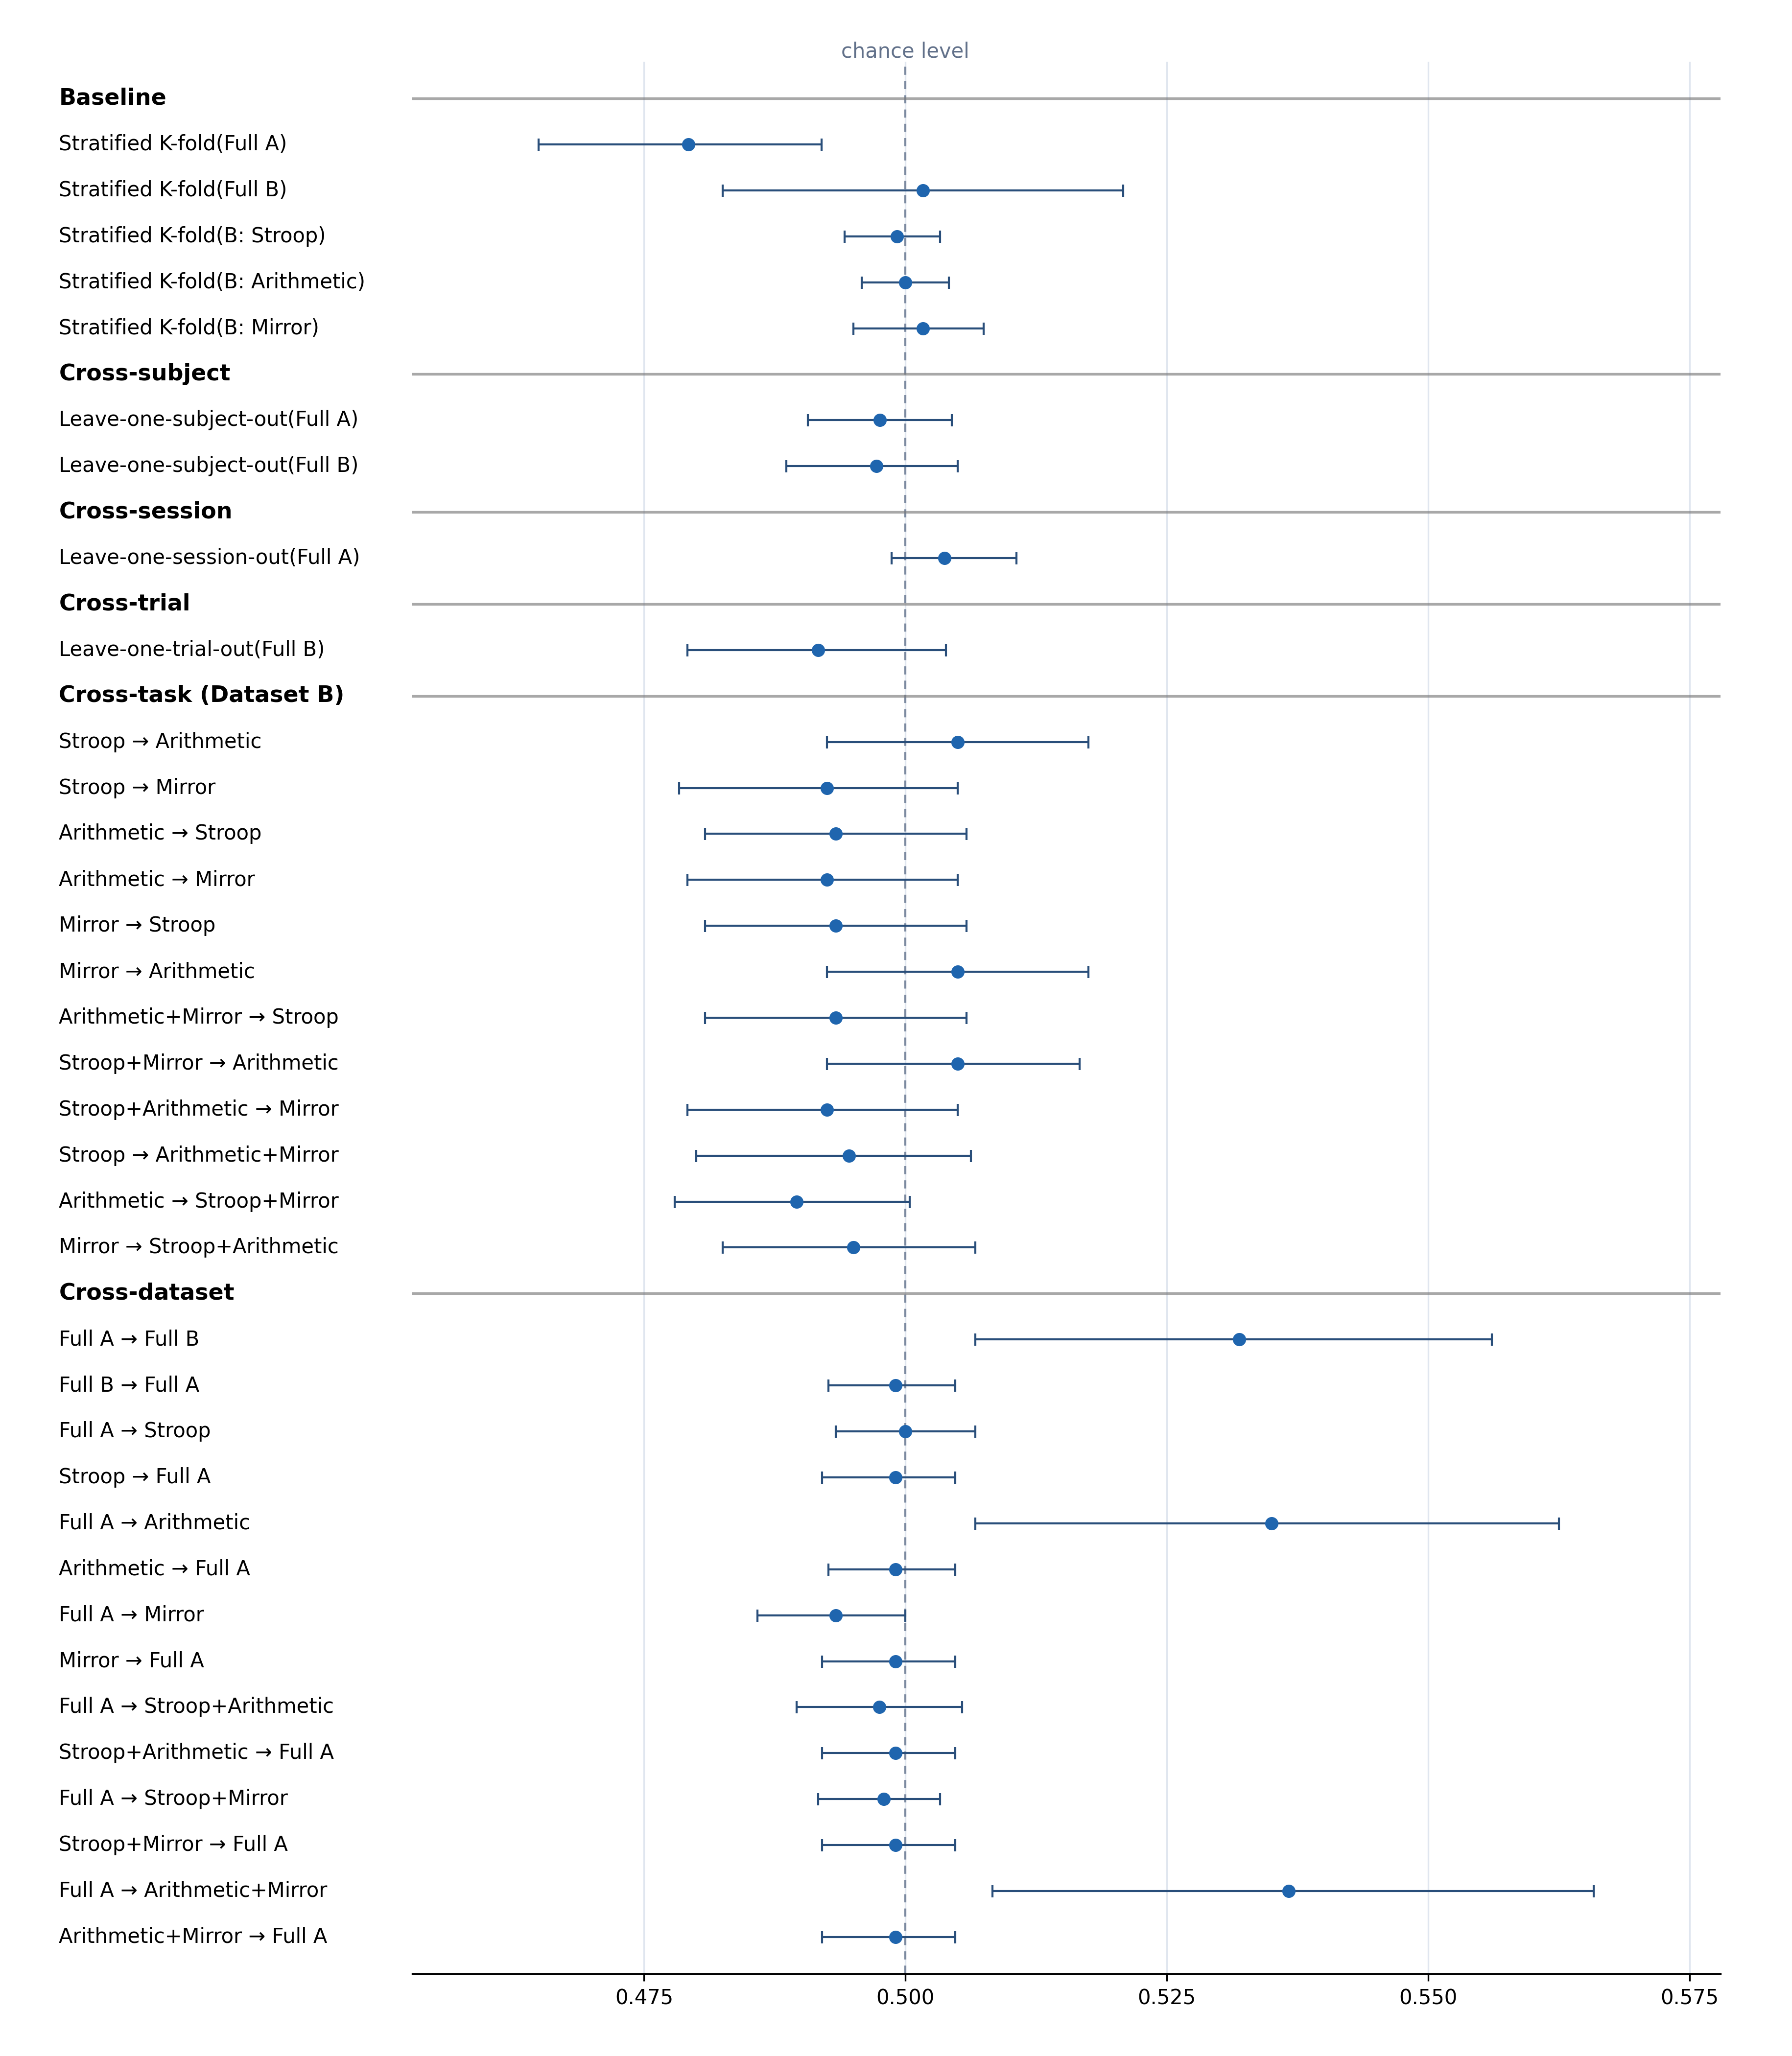
\includegraphics[width=\textwidth,height=0.88\textheight,keepaspectratio]{figures/supplementary/S4_fig_shallownet_all_scenarios.png}
\end{center}

\clearpage
\noindent\textbf{S3 Fig. EEGConformer balanced accuracy across validation protocols.}
\begin{center}
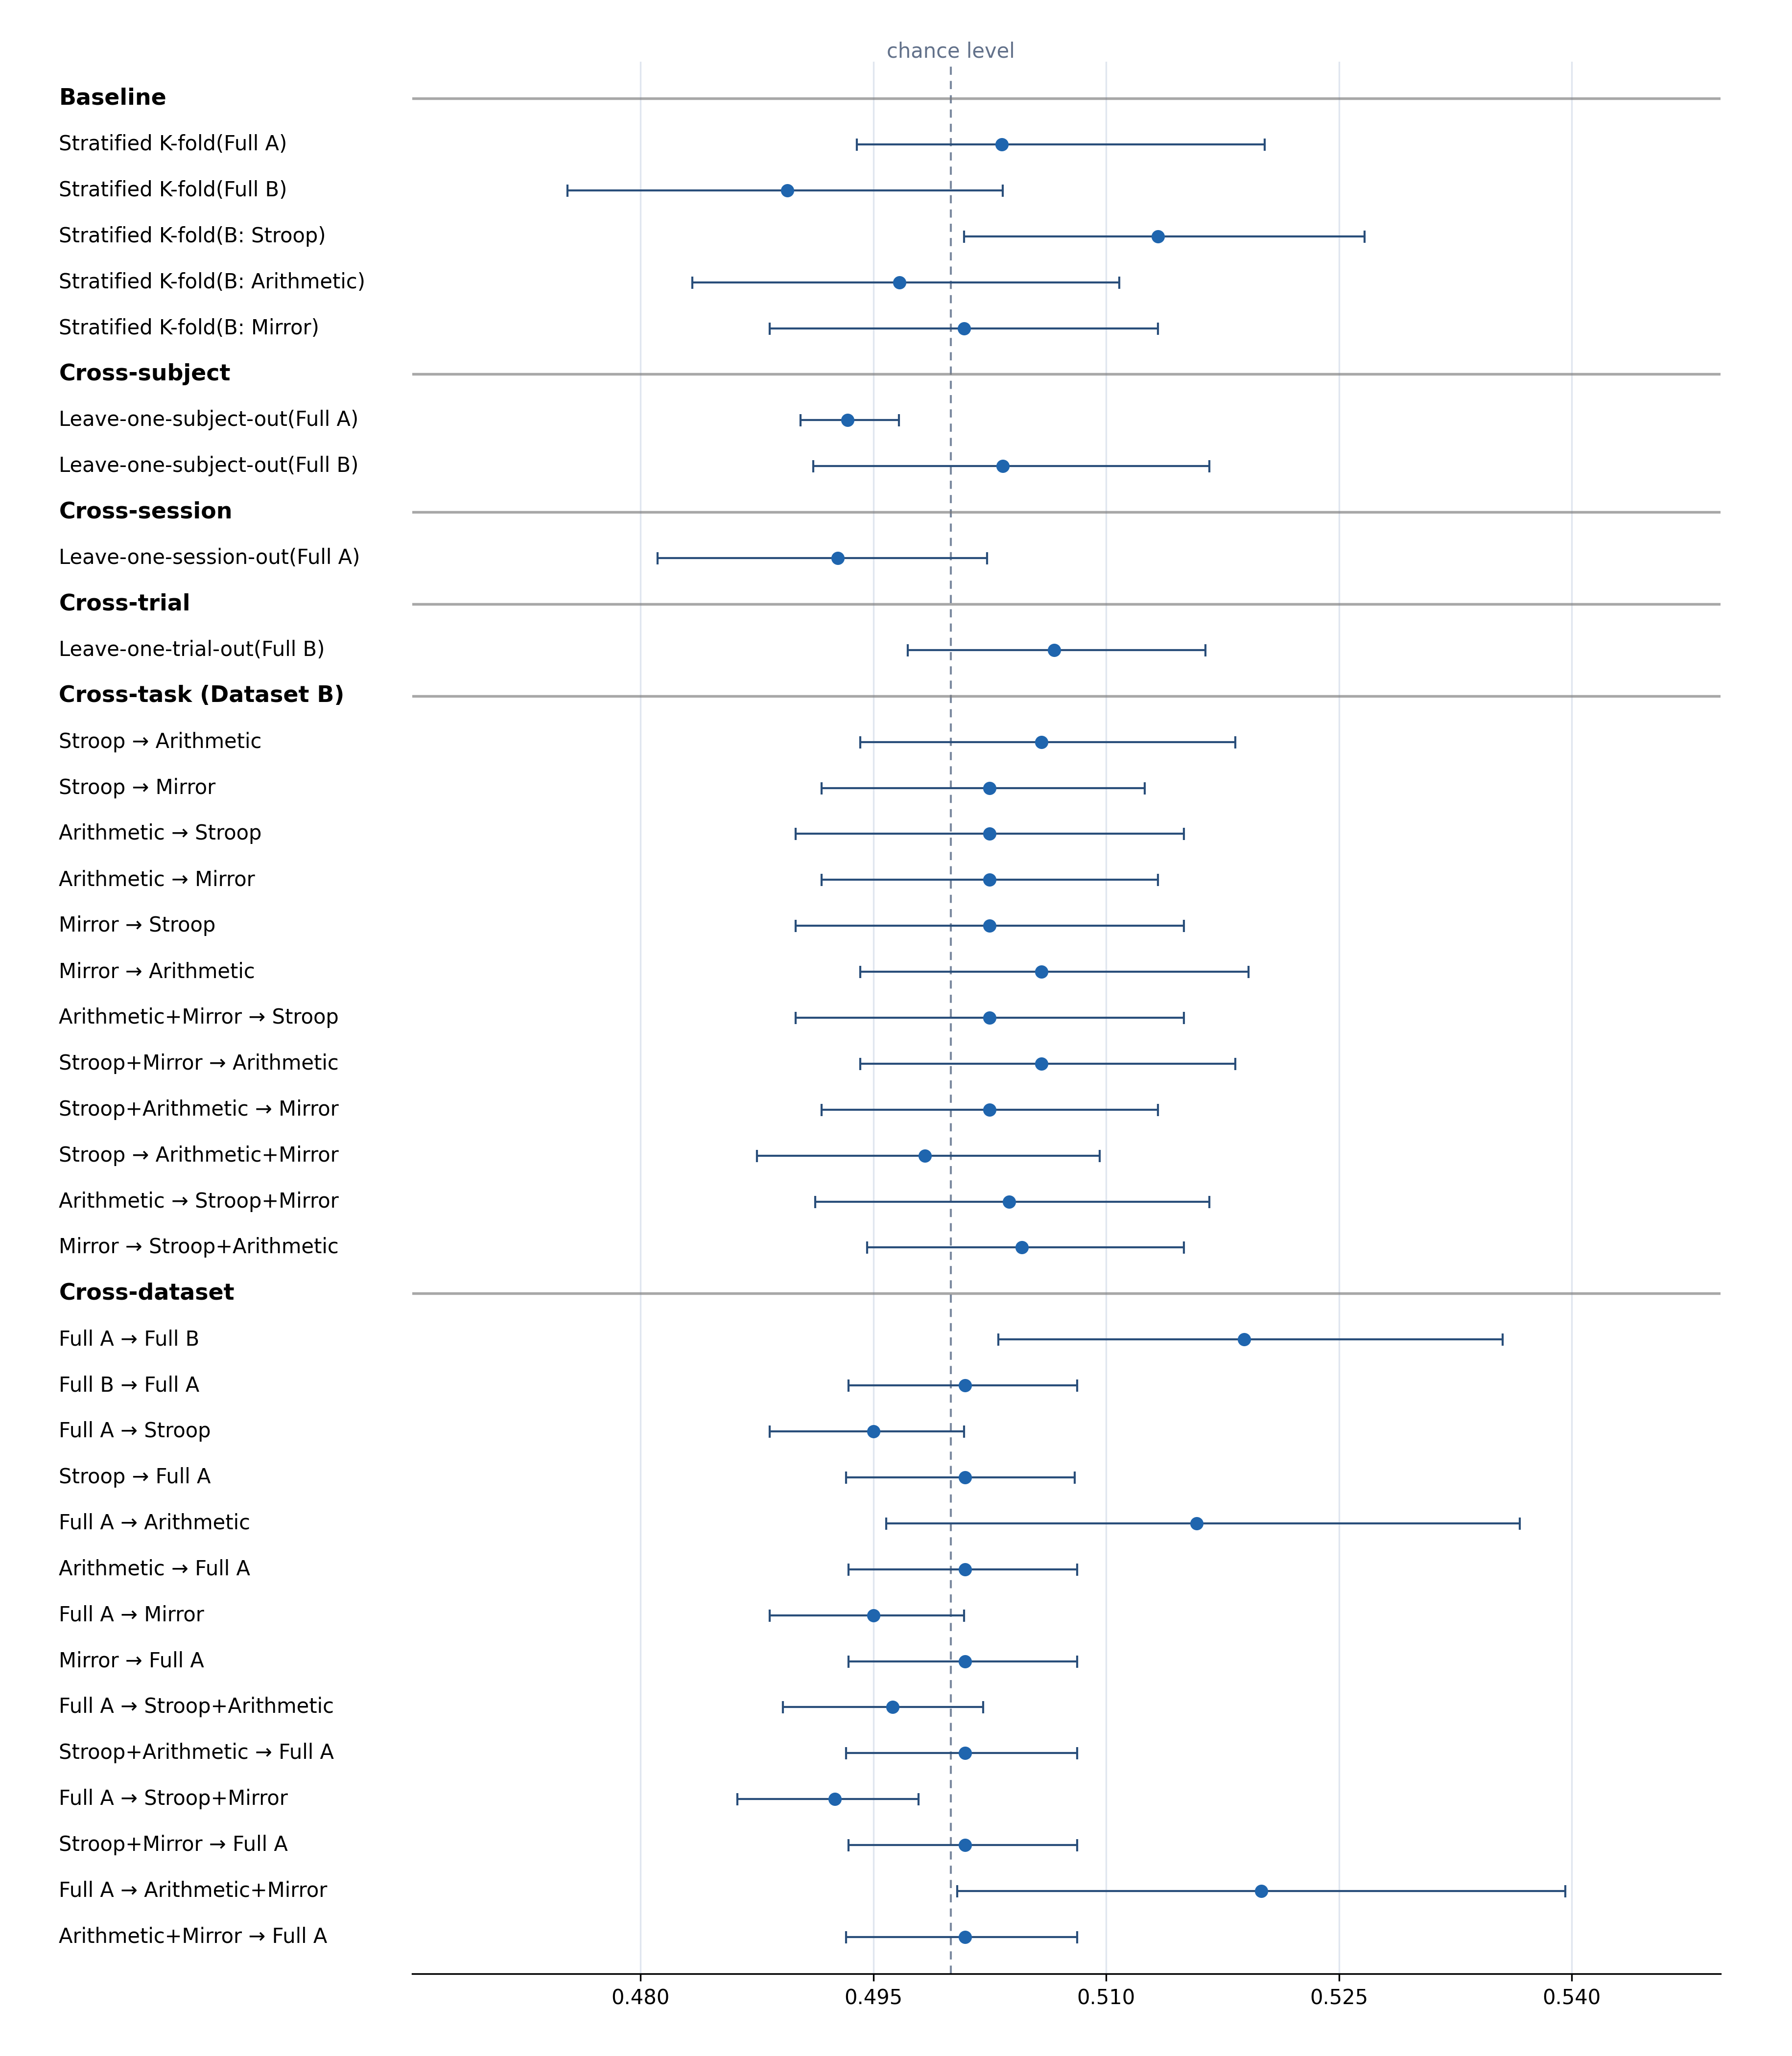
\includegraphics[width=\textwidth,height=0.88\textheight,keepaspectratio]{figures/supplementary/S5_fig_eegconformer_all_scenarios.png}
\end{center}

\paragraph*{S1 Table.}
\label{S1_Table_Logistic}
{\bf Logistic-regression performance metrics across all experimental scenarios.}

\paragraph*{S2 Table.}
\label{S2_Table_XGBoost}
{\bf XGBoost performance metrics across all experimental scenarios.}

\paragraph*{S3 Table.}
\label{S3_Table_EEGNet}
{\bf EEGNet performance metrics across all experimental scenarios.}

\paragraph*{S4 Table.}
\label{S4_Table_ShallowNet}
{\bf ShallowFBCSPNet performance metrics across all experimental scenarios.}

\paragraph*{S5 Table.}
\label{S5_Table_EEGConformer}
{\bf EEGConformer performance metrics across all experimental scenarios.}

\paragraph*{S6 Table.}
\label{S6_Table}
{\bf Preprocessing, feature extraction and model configuration.}
\textbf{[TODO --- Regenerate this table for the current model set.]}

Full parameter values for every preprocessing, feature extraction and model
step, as recorded in the versioned experiment configuration. Continuous-signal
filtering: band-pass 0.5--45\,Hz, 50\,Hz notch, average reference. Artifact removal: FastICA, 0.99 explained-variance component
count, fit on data band-passed 1--45\,Hz, EOG-proxy channels F3/F4/F7/F8 with
threshold 2.4, random state 42. Epoching: 5\,s windows with 0.5\,s overlap
over a common 12-channel montage (F3, F4, F7, F8, FC5, FC6, O1, O2, P7, P8,
T7, T8). Record selection: sessions with \texttt{session\_role=habituation}
or \texttt{session\_quality=incomplete} excluded prior to Stage 1. Feature
extraction (spectral configuration): log band power in five bands
(0.5--4, 4--8, 8--13, 13--30, 30--45\,Hz) plus spectral entropy per channel.
Models: the six configurations named in the Models subsection, with the feature
scaler fitted inside the pipeline on the training fold only. Global random seed: 42. Validation protocols: stratified
group $K$-fold baseline grouped by physical recording, cross-subject,
cross-session (session-documented dataset only) and cross-trial
(repeated-task dataset) group-aware splits, cross-dataset and leave-one-
subject-out cross-task transfer. No data-driven hyperparameter tuning was
performed. Hyperparameters were fixed a priori for the benchmark comparison.

\end{document}
